\chapter{Exercise 1}

All tasks are implemented in Python using the SciPy-stack.
Image data is parsed into Numpy arrays and processed using a combination of built-in functions from SciPy and functions we have implemented ourselves.

\section*{Task 3 - Basic Image Manipulation}

\subsection*{1 - Correct an image using a flatfield image}

Listing \ref{flatfield} shows the two relevant functions implemented for this task.
For the complete implementation including reading the image files and saving/showing the end result, see the file \texttt{flatfield.py}.

\begin{lstlisting}[language=Python, label=flatfield, caption=Flatfield image correction]
def normalize_bw(img_matrix):
    return map(lambda row: map(lambda val: val / 255, row), img_matrix)


def correct_with_flatfield(img, flatfield):
    corrected = deepcopy(img)
    for y, (a_row, b_row) in enumerate(zip(img, flatfield)):
        for x, (a_px, b_px) in enumerate(zip(a_row, b_row)):
            corrected[y][x] = a_px / b_px

    return corrected
\end{lstlisting}

\begin{figure}[h!]
    \centering
    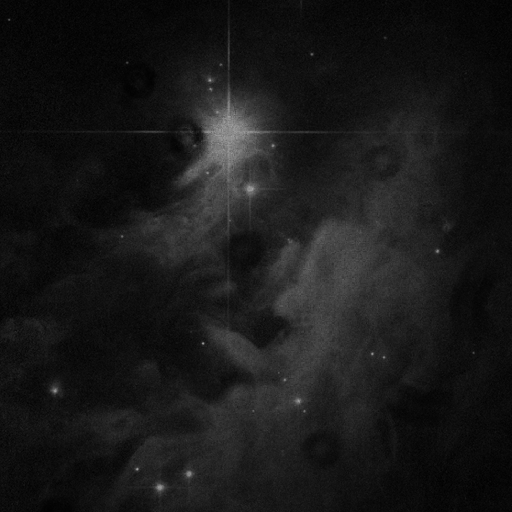
\includegraphics[width=5cm]{../LAB1/img/disturbed_potw1144a.png}
    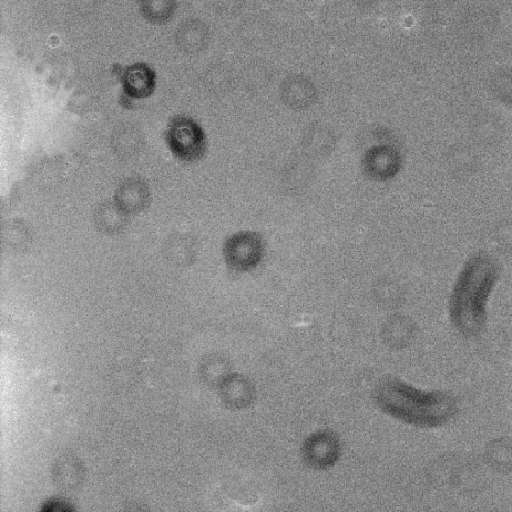
\includegraphics[width=5cm]{../LAB1/img/flatfieldimage.png}
    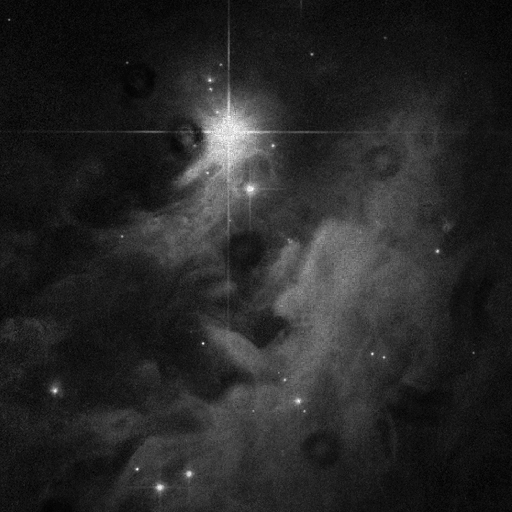
\includegraphics[width=5cm]{../LAB1/output/disturbed_potw1144a.png}
    \caption{From the left: original, flat-field image, corrected}
\end{figure}

\subsection*{2 - Speculation}

When performing flat-field correction we want to compensate for imperfections of the detector by scaling the intensity value of a pixel by scaling with the intensity value of the same pixel in the flat-field image.
If we did this by subtraction, i.e original\_pixel\_intensity - flat\_field\_intensity, we could end up with negative values.


\section*{Task 4 - Point processing}

\subsection*{1 - Intensity Transform}

%\clearpage
\section*{Task 4 - Point Processing}

\subsection*{Intensity transform}

The gamma correction is done by applying the function $px_{new} = {px_{old}}^{\gamma}$.
Because we're operating with input and output that is integers in the [0, 255] range, not floating point numbers in the [0, 1] range, we need to take this into consideration for the calculation.
\begin{lstlisting}[language=Python, label=gamma_correction, caption=Gamma correction]
def pixel_wise_transform(matrix, fun):
    '''
    applies fun(px) to every px in the 2d matrix
    '''
    return np.asarray(map(lambda row: map(lambda px: fun(px), row), matrix))


def gamma_correct(matrix, gamma=1.0):
    '''
    applies the gamma correction function (px)^(gamma) to the matrix
    '''
    return pixel_wise_transform(matrix, lambda px: int(255 * ((px / 255) ** gamma)))
\end{lstlisting}

\begin{figure}[h!]
    \centering
    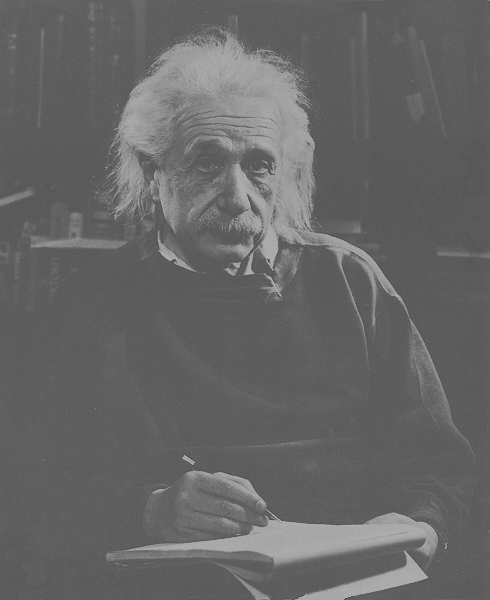
\includegraphics[width=5cm]{../LAB1/img/einstein_lowcontrast.png}
    \includegraphics[width=5cm]{../LAB1/output/gamma_einstein_lowcontrast.png}
    \includegraphics[width=5cm]{../LAB1/output/stretched_gamma_einstein_lowcontrast.png}
    \caption{From the left: einstein\_lowcontrast.png, gamma corrected, input range stretched then gamma corrected.}
\end{figure}


\begin{lstlisting}[language=Python, label=input_range, caption=Input range stretching]
def minmax_2d(matrix):
    '''
    returns the minimum and maximum value of a 2d matrix
    '''
    return map(lambda f: f(f(matrix, key=lambda x: f(x))), (min, max))


def stretch_range(matrix):
    '''
    stretches the range of matrix to [0, 255]
    '''
    m_min, m_max = minmax_2d(matrix)
    return pixel_wise_transform(matrix, lambda px: int((px - m_min) / ((m_max - m_min) / 255)))
\end{lstlisting}

\subsection*{Histogram equalization}


\section*{Task 5 - Noise}

\subsection*{1 - Salt \& Pepper noise}

Since SciPy, and PIL specifically, doesn't provide an \texttt{imnoise}-function, this task had to be implemented manually. \ref{salt-and-pepper}

\begin{lstlisting}[language=Python, label=salt-and-pepper, caption=Salt \& pepper noise]
def salt_and_pepper_noise(matrix, density):
    return pixel_wise_transform(matrix, lambda px: np.random.randint(2) if np.random.random() < density else px)

# pixel_wise_transform implementation
def pixel_wise_transform(matrix, fun):
    '''
    applies fun(px) to every px in the 2d matrix
    '''
    return np.asarray(map(lambda row: map(lambda px: fun(px), row), matrix))
\end{lstlisting}

